\documentclass[a4paper,man,biblatex]{apa6}
\usepackage[american]{babel}
\usepackage{float}
\usepackage{csquotes}
\usepackage{siunitx}
\usepackage[backend=biber]{biblatex}
\usepackage[document]{ragged2e}
\setlength{\RaggedRightParindent}{0.5in}
\addbibresource{../references/references.bib}
\usepackage{graphicx}
\graphicspath{{./img/}}
\usepackage{url}
\usepackage{xpatch}
\usepackage{siunitx}
\xpatchbibdriver{online}
  {\printfield{entrysubtype}}
  {\printfield{entrysubtype}%
   \newunit\newblock
   \printfield{note}}
  {}
  {}

\renewcommand{\abstract}[1]{}

\title{Research Summary \& Draft Thesis}
\shorttitle{Research Summary \& Draft Thesis}
\author{Armant Touche}
\affiliation{Portland State University}
\date{\today}

\begin{document}
\thispagestyle{otherpage}
\setcounter{biburllcpenalty}{7000}
\setcounter{biburlucpenalty}{8000}

%\maketitle

\section{Introduction} In this research paper, I will be describing how researchers measure "human disturbance" in regard to streamflow variability, the validity of the "human disturbance" index, and current cases of variability having an affect in the Southwest region of the United States. The "human disturbance" index is measurement tool used by the United States Environmental Protection Agency (USEPA) to measure the amount of disturbance present in watershed regions across the nation \autocite{falcone_2016}. The reason for needing the index is to use this measurement, along with other variables, to track the behavior of these hydrological systems. Changes in hydrological systems in the Continental United States (CONUS) have caused some negative outcomes where one being an increase in floods in some regions \autocite{rice_2016}. A regional example of a negative outcome from increased streamflow variability is the increasing number of floods in California \autocite{standford_2020}. The scale of variability is still being studied since previous methods used datasets that contained redundancies, which decreased accuracy but \textcite{falcone_2016} described the best approach to accurately classifying. There is a relationship between streamflow variability and both water resource availability and management \autocite{rice_2016}. For present and future studies in relation to hydrological systems, understanding the previously mentioned relationship is crucial to measure human activity and the impact of the side effects from such activity in order to positively manage water resources here in the CONUS and elsewhere in the world.
\medskip

\section{Data Analysis} 
\makebox[0pt][l]{%
\begin{minipage}{\textwidth}
            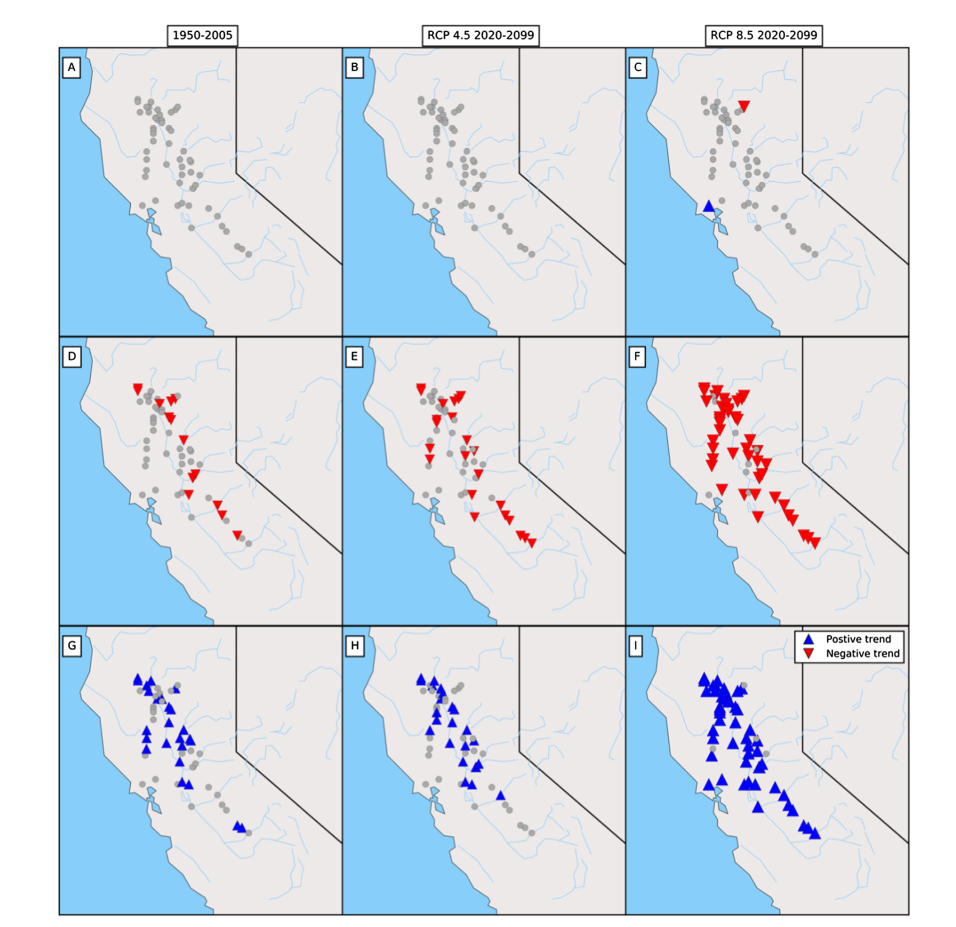
\includegraphics[width=.75\textwidth]{stream_flow_cali}
            \captionof{figure}{statistically significant trends in the annual mean (panel a-c), annual minima (panel d-f) and annual maxima (panel g-i) flows over northern california. left panels summarize the results for the historical baseline period. middle and right panels represent change in the projection period under the rcp 4.5 and 8.5 scenarios, respectively.\label{fig:stream_flow}}
    \end{minipage}
}
\medskip
\par To better understand the negative outcomes from increased streamflow variability and increasingly warming climate, the \textcite{mallakpour_2018} study reported streamflow minimum and maximum annual streamflows mean (\si{\cubic\meter\per\second}) comparing watershed in Northern California. In ~\ref{fig:stream_flow}, notice the min. streamflow values (red-down arrows) in panels D-F. In D-panel, there is more reports on negative trend in streamflow values from 1950-2005 which means that rivers and such are displaying a decreasing mean during the dry seasons and in G-panel, during the wet season, there is increase in the mean. The increase in mean during the wet-season promotes more floods and decrease in mean during dry-season promotes more droughts \autocite{mallakpour_2018}.
\section{Relevance} 

\section{Results} 

\section{Conclusion}  

\printbibliography

\end{document}
